\section{VANET 환경에서 안전한 차량 통신을 위한 프로토콜}
    \textbf{박영호. (2010). VANET 환경에서 안전한 통신을 위한 차량 등록 프로토콜. 한국산업정보학회논문지, 15(4), 1-5.}
    \\\\
    VANET은 원활한 교통 소통, 사고 방지 등 여러가지 편리한 기능을 제공하지만 Ad-hoc 네트워크에 기반을 두고 있기 때문에 추가적인 보안 요구 사항이 존재한다. 특히, VANET의 안전한 활용을 위해서는 가입자를 확인하고 메시지 변조를 일으킬 수 있는 악의적인 가입자를 막는 인증이 필요하다. VANET은 차량이 고속으로 이동하는 빠르게 변화하는 망이기 때문에 연산 부하가 적은 인증 프로토콜을 구성해야한다. 이 연구는 일방향 함수와 EOR 연산을 이용하여 차량 등록 인증을 수행하는 프로토콜을 제안한다. \\
    \vspace{-4mm}
        \begin{figure}[!h]\centering
    		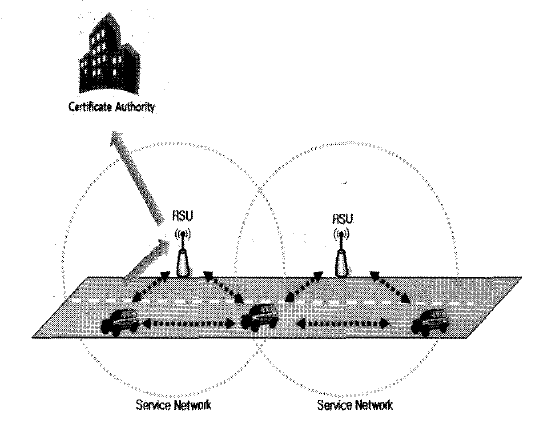
\includegraphics[width=.65\textwidth]{image/week13/4-1.png}
    		\caption{\small VANET 환경에서의 차량 등록 프로토콜 적용 시나리오}
    		\vspace{-10pt}
        \end{figure}
    
    이 프로토콜은 인증센터가 차량을 인증하는 단방향 차량 등록 인증 프로토콜이다. V2I(Vehicle to Infrastructure)의 확장된 개념으로 차량이 노변장치(RSU, road side unit)를 거쳐 인증센터(CA, Certificate Authority)와 통신하여 통신상에 필요한 차량 인증을 제공한다. 차량과 인증 센터간의 공유된 키 검증자를 통해 CA가 생성한 세션 키의 안전한 분배가 이루어지게 되고 세션 키를 통해 생성한 인증 값과 차량의 인증 결과 값을 비교 검증하여 동일한 값일 경우 차량 등록 인증하게 된다. \\
    제안한 차량 등록 프로토콜의 안정성 및 성능 분석 결과, 위장 공격, 재전송 공격, MITM 공격, 메시지 변조 공격으로부터 사용자를 보호할 수 있음을 보였다.